\specialchapter{\texorpdfstring{PLATE V. SYSTEM OF TYPE \(E_{6}\)}{PLATE V. SYSTEM OF TYPE E\_6}}

\begin{enumerate}
\def\labelenumi{(\Roman{enumi})}
\tightlist
\item
  V is the subspace of \(E = R^{8}\) consisting of the points whose coordinates \((\xi_{i})\) are such that \(\xi_{6} = \xi_{7} = -\xi_{8}\) . Roots: \(\pm\varepsilon_{i} \pm \varepsilon_{j} (1 \leqslant i < j \leqslant 5)\) ,
\end{enumerate}

\[
\pm \frac {1}{2} (\varepsilon_ {8} - \varepsilon_ {7} - \varepsilon_ {6} + \sum_ {i = 1} ^ {5} (- 1) ^ {\nu (i)} \varepsilon_ {i}) \text {with} \sum_ {i = 1} ^ {5} \nu (i) \text {even.}
\]

Number of roots: n = 72.

\begin{enumerate}
\def\labelenumi{(\Roman{enumi})}
\setcounter{enumi}{1}
\tightlist
\item
Basis: \(\alpha_{1} = \frac{1}{2} (\varepsilon_{1} + \varepsilon_{8}) - \frac{1}{2} (\varepsilon_{2} + \varepsilon_{3} + \varepsilon_{4} + \varepsilon_{5} + \varepsilon_{6} + \varepsilon_{7}),\alpha_{2} = \varepsilon_{1} + \varepsilon_{2},\alpha_{3} =\) \(\varepsilon_2 - \varepsilon_1,\alpha_4 = \varepsilon_3 - \varepsilon_2,\alpha_5 = \varepsilon_4 - \varepsilon_3,\alpha_6 = \varepsilon_5 - \varepsilon_4.\) Positive roots: \(\pm \varepsilon_i + \varepsilon_j\) \(1\leqslant i <   j\leqslant 5)\)
\end{enumerate}

\[
\frac {1}{2} \left(\varepsilon_ {8} - \varepsilon_ {7} - \varepsilon_ {6} + \sum_ {i = 1} ^ {5} (- 1) ^ {\nu (i)} \varepsilon_ {i}\right) \text {with} \sum_ {i = 1} ^ {5} \nu (i) \text {even}.
\]

Positive roots with at least one coefficient \(\geqslant 2\) (we denote the root \(a\alpha_{1} + b\alpha_{2} + c\alpha_{3} + d\alpha_{4} + e\alpha_{5} + f\alpha_{6}\) ) by \({ }^{a c d e f}_{b})^{13}\) :

\[
\begin{array}{c c c c c c} 0   1   2   1   0 & 1   1   2   1   0 & 0   1   2   1   1 & 1   2   2   1   0 & 1   1   2   1   1 & 0   1   2   2   1 \\ 1 & 1 & 1 & 1 & 1 & 1 \\ 1   2   2   1   1 & 1   1   2   2   1 & 1   2   2   2   1 & 1   2   3   2   1 & 1   2   3   2   1 \\ 1 & 1 & 1 & 1 & 2 \end{array}
\]

\begin{enumerate}
\def\labelenumi{(\Roman{enumi})}
\setcounter{enumi}{2}
\item
  Coxeter number: \(h = 12\) .
\item
  Highest root:
\end{enumerate}

\[
\begin{array}{r l} \tilde {\alpha} & = \frac {1}{2} (\varepsilon_ {1} + \varepsilon_ {2} + \varepsilon_ {3} + \varepsilon_ {4} + \varepsilon_ {5} - \varepsilon_ {6} - \varepsilon_ {7} + \varepsilon_ {8}) \\ & = \alpha_ {1} + 2 \alpha_ {2} + 2 \alpha_ {3} + 3 \alpha_ {4} + 2 \alpha_ {5} + \alpha_ {6} = \omega_ {2}. \end{array}
\]

Completed Dynkin graph:

\pandocbounded{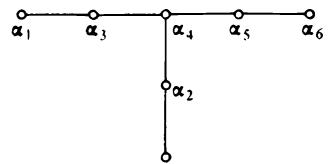
\includegraphics[keepaspectratio]{images/part002_985a73c0.jpg}}

\begin{enumerate}
\def\labelenumi{(\Alph{enumi})}
\setcounter{enumi}{21}
\tightlist
\item
  \(R^{\prime} = R.\)
\end{enumerate}

\[
  \Phi_ {\mathrm{R}} (x, y) = (x | y) / 24, \quad \gamma (\mathrm{R}) = 144.
\]

\begin{enumerate}
\def\labelenumi{(\Roman{enumi})}
\setcounter{enumi}{5}
\tightlist
\item
  Fundamental weights:
\end{enumerate}

\[
\begin{array}{l} \omega_ {1} = \frac {2}{3} (\varepsilon_ {8} - \varepsilon_ {7} - \varepsilon_ {6}) = \frac {1}{3} (4 \alpha_ {1} + 3 \alpha_ {2} + 5 \alpha_ {3} + 6 \alpha_ {4} + 4 \alpha_ {5} + 2 \alpha_ {6}) \\ \omega_ {2} = \frac {1}{2} (\varepsilon_ {1} + \varepsilon_ {2} + \varepsilon_ {3} + \varepsilon_ {4} + \varepsilon_ {5} - \varepsilon_ {6} - \varepsilon_ {7} + \varepsilon_ {8}) \\ \quad = \alpha_ {1} + 2 \alpha_ {2} + 2 \alpha_ {3} + 3 \alpha_ {4} + 2 \alpha_ {5} + \alpha_ {6} = \tilde {\alpha} \\ \omega_ {3} = \frac {5}{6} (\varepsilon_ {8} - \varepsilon_ {7} - \varepsilon_ {6}) + \frac {1}{2} (- \varepsilon_ {1} + \varepsilon_ {2} + \varepsilon_ {3} + \varepsilon_ {4} + \varepsilon_ {5}) \\ \quad = \frac {1}{3} (5 \alpha_ {1} + 6 \alpha_ {2} + 10 \alpha_ {3} + 12 \alpha_ {4} + 8 \alpha_ {5} + 4 \alpha_ {6}) \\ \omega_ {4} = \varepsilon_ {3} + \varepsilon_ {4} + \varepsilon_ {5} - \varepsilon_ {6} - \varepsilon_ {7} + \varepsilon_ {8} \\ \quad = 2 \alpha_ {1} + 3 \alpha_ {2} + 4 \alpha_ {3} + 6 \alpha_ {4} + 4 \alpha_ {5} + 2 \alpha_ {6} \\ \omega_ {5} = \frac {2}{3} (\varepsilon_ {8} - \varepsilon_ {7} - \varepsilon_ {6}) + \varepsilon_ {4} + \varepsilon_ {5} \\ \quad = \frac {1}{3} (4 \alpha_ {1} + 6 \alpha_ {2} + 8 \alpha_ {3} + 12 \alpha_ {4} + 10 \alpha_ {5} + 5 \alpha_ {6}) \\ \omega_ {6} = \frac {1}{3} (\varepsilon_ {8} - \varepsilon_ {7} - \varepsilon_ {6}) + \varepsilon_ {5} \\ \quad = \frac {1}{3} (2 \alpha_ {1} + 3 \alpha_ {2} + 4 \alpha_ {3} + 6 \alpha_ {4} + 5 \alpha_ {5} + 4 \alpha_ {6}). \end{array}
\]

\begin{enumerate}
\def\labelenumi{(\Roman{enumi})}
\setcounter{enumi}{6}
\tightlist
\item
  Sum of the positive roots:
\end{enumerate}

\[
\begin{array}{l} 2 \rho = 2 (\varepsilon_ {2} + 2 \varepsilon_ {3} + 3 \varepsilon_ {4} + 4 \varepsilon_ {5} + 4 (\varepsilon_ {8} - \varepsilon_ {7} - \varepsilon_ {6})) \\ = 2 (8 \alpha_ {1} + 11 \alpha_ {2}) + 15 \alpha_ {3} + 21 \alpha_ {4} + 15 \alpha_ {5} + 8 \alpha_ {6}). \end{array}
\]

\begin{enumerate}
\def\labelenumi{(\Roman{enumi})}
\setcounter{enumi}{7}
\tightlist
\item
  P(R)/Q(R) is isomorphic to Z/3Z.
\end{enumerate}

Connection index: 3.

\begin{enumerate}
\def\labelenumi{(\Roman{enumi})}
\setcounter{enumi}{8}
\item
  Exponents: 1, 4, 5, 7, 8, 11.
\item
  Order of W(R): \(2^{7}.3^{4}.5\) .
\item
  \(\mathrm{A}(\mathrm{R}) = \mathrm{W}(\mathrm{R}) \times \{1, -1\}\) ; \(w_0\) transforms \(\alpha_1, \alpha_2, \alpha_3, \alpha_4, \alpha_5, \alpha_6\) , respectively, into \(-\alpha_6, -\alpha_2, -\alpha_5, -\alpha_4, -\alpha_3, -\alpha_1\) .
\item
  The non-identity element of \(\mathrm{A}(\mathbb{R}) / \mathrm{W}(\mathbb{R})\) defines the automorphism \(x \mapsto -x\) of \(\mathrm{P}(\mathbb{R}) / \mathrm{Q}(\mathbb{R})\) .
\end{enumerate}

The group of automorphisms of the completed Dynkin diagram is isomorphic to \(S_{3}\) ; its elements of order 3 are induced by the two non-trivial elements of \(P(R^{-})/Q(R^{-})\) .

\[
\left( \begin{array}{c c c c c c} 2 & 0 & - 1 & 0 & 0 & 0 \\ 0 & 2 & 0 & - 1 & 0 & 0 \\ - 1 & 0 & 2 & - 1 & 0 & 0 \\ 0 & - 1 & - 1 & 2 & - 1 & 0 \\ 0 & 0 & 0 & - 1 & 2 & - 1 \\ 0 & 0 & 0 & 0 & - 1 & 2 \end{array} \right)
\]

\begin{enumerate}
\def\labelenumi{(\Roman{enumi})}
\setcounter{enumi}{12}
\tightlist
\item
  Cartan matrix:
\end{enumerate}

